\chapter{Interpolation, Discount Factors and Forward Rates}\label{interpolation---practical-lesson-3}

In this Chapter we will start to see the first applications of \texttt{python} to financial calculations.
In particular we will consider discount curves and forward rates, implementing the first utilities that will fill our financial module.
In doing so we will review a widely used mathematical tool: \emph{interpolation}.

\section{Linear Interpolation}\label{linear-interpolation}

Consider to have few data points, obtained by sampling or experimenting. These points represent the values of a not well known function \(f(x)\), where \(x\) is an independent variable (e.g.~in recording a trip: distances at certain times, \(d = f(t)\)).

It may be necessary to estimate values of the function $f$ at values for which we don't have samples.
Interpolation is a method of "constructing" new points within the range of the known data.

Let's clarify the technique with an example.
Assume you are going on holidays by car and that luckily there isn't much traffic so that you can drive at constant speed (which gives a linear relation between traveled space and time i.e.~\(s = v \cdot t\), which means that if you plot the distances \(s\) as a function of the time \(t\) you get a line with slope \(v\)), see Fig.~\ref{fig:samples_for_interpolation}.

\begin{figure}
  \centering
  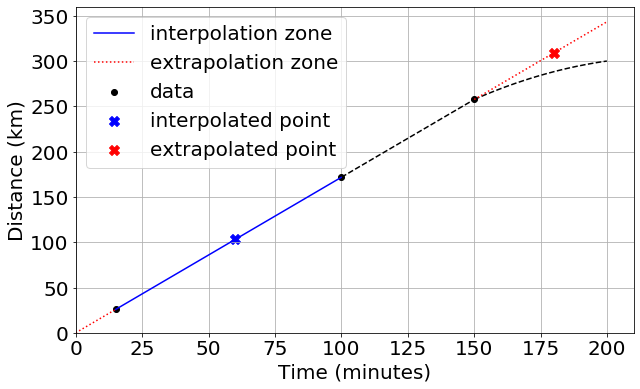
\includegraphics[width=0.7\textwidth]{figures/interp_example1.png}
  \caption{An example of sampling of traveled distances at some time. The red point shows an additional sample taken after the trip velocity has been reduced.}
  \label{fig:samples_for_interpolation}
\end{figure}

Given two samples of the car traveled distance \(s_1\) and \(s_2\) taken at two different times \(t_1\) and \(t_2\) you can linearly interpolate to find your position at different times using the following relations:

\begin{equation}
s = (1 - w)\cdot s_1 + w \cdot s_2
\end{equation}
where $t$ is a generic time at which we want to know the distance $s$ and \(w = \cfrac{t - t_1}{t_2 - t_1}\).

\begin{attention}
\subsubsection{Derivation}
The equation of a line for two points
\((t_1, s_1)\) and \((t_2, s_2)\) can be written as:

\begin{equation}
\frac{t - t_1}{t_2 - t_1} = \frac{s - s_1}{s_2 - s_1}
\end{equation}

Setting again \(w = \cfrac{t - t_1}{t_2 - t_1}\) and solving for \(s\) we find the desired solution:

\begin{equation}(s_2 - s_1)\cdot w = s - s_1\quad\implies\quad s = (1 - w)\cdot s_1 + w \cdot s_2
\end{equation}

This formula can also be understood as a weighted average where the weights are inversely related to the distance from the end points to the unknown point ($w_1 = (1 - w) = \cfrac{t_2 - t}{t_2 -t_1}, w_2 = w$), the closer point has more influence than the farther point.
\end{attention}

Back to our example, if
\(s_1 = 25.75~\mathrm{km}\;(@t_1 = 15~\mathrm{min})\) and
\(s_2 = 171.7~\mathrm{km}\;(@t_2 = 100~\mathrm{min})\) let's find distance traveled in 1 hour (interpolation):

\begin{codebox}
\begin{Verbatim}[commandchars=\\\{\}]
\PY{n}{s\PYZus{}1} \PY{o}{=} \PY{l+m+mf}{25.75} \PY{c+c1}{\PYZsh{} distance in km}
\PY{n}{t\PYZus{}1} \PY{o}{=} \PY{l+m+mi}{15}    \PY{c+c1}{\PYZsh{} elapsed time in minutes}
\PY{n}{s\PYZus{}2} \PY{o}{=} \PY{l+m+mf}{171.7}
\PY{n}{t\PYZus{}2} \PY{o}{=} \PY{l+m+mi}{100}

\PY{n}{t} \PY{o}{=} \PY{l+m+mi}{60}

\PY{n}{w} \PY{o}{=} \PY{p}{(}\PY{n}{t} \PY{o}{\PYZhy{}} \PY{n}{t\PYZus{}1}\PY{p}{)}\PY{o}{/}\PY{p}{(}\PY{n}{t\PYZus{}2} \PY{o}{\PYZhy{}} \PY{n}{t\PYZus{}1}\PY{p}{)}
\PY{n}{s} \PY{o}{=} \PY{p}{(}\PY{l+m+mi}{1} \PY{o}{\PYZhy{}} \PY{n}{w}\PY{p}{)}\PY{o}{*}\PY{n}{s\PYZus{}1} \PY{o}{+} \PY{n}{w}\PY{o}{*}\PY{n}{s\PYZus{}2}

\PY{n+nb}{print} \PY{p}{(}\PY{l+s+s2}{\PYZdq{}}\PY{l+s+si}{\PYZob{}:.1f\PYZcb{}}\PY{l+s+s2}{ km}\PY{l+s+s2}{\PYZdq{}}\PY{o}{.}\PY{n}{format}\PY{p}{(}\PY{n}{s}\PY{p}{)}\PY{p}{)}

103.0 km
\end{Verbatim}
\end{codebox}

Always interpret critically your results to guess if they make sense or not. In the previous example we certainly expected something between 25.75 and 171.7~km (our range ends) furthermore since we are looking for the distance at a time which is almost halfway the interval, the result will be somehow in the middle or around 98.6~km. This is indeed more or less what we have got.
This simple reasoning should be applied every time you have a result to quickly judge it.

If we believe the relation between our variable stays the same ($f(t)$ still linear), we can use the same formula to \emph{extrapolate} values \emph{outside} our initial sample. For example if we keep the same constant velocity in our trip we could check the distance traveled after 3 hours:

\begin{codebox}
\begin{Verbatim}[commandchars=\\\{\}]
\PY{n}{s\PYZus{}1} \PY{o}{=} \PY{l+m+mf}{25.75} \PY{c+c1}{\PYZsh{} distance in km}
\PY{n}{t\PYZus{}1} \PY{o}{=} \PY{l+m+mi}{15}    \PY{c+c1}{\PYZsh{} elapsed time in minutes}
\PY{n}{s\PYZus{}2} \PY{o}{=} \PY{l+m+mf}{171.7}
\PY{n}{t\PYZus{}2} \PY{o}{=} \PY{l+m+mi}{100}

\PY{n}{t} \PY{o}{=} \PY{l+m+mi}{180}

\PY{n}{w} \PY{o}{=} \PY{p}{(}\PY{n}{t} \PY{o}{\PYZhy{}} \PY{n}{t\PYZus{}1}\PY{p}{)}\PY{o}{/}\PY{p}{(}\PY{n}{t\PYZus{}2} \PY{o}{\PYZhy{}} \PY{n}{t\PYZus{}1}\PY{p}{)}
\PY{n}{s} \PY{o}{=} \PY{p}{(}\PY{l+m+mi}{1} \PY{o}{\PYZhy{}} \PY{n}{w}\PY{p}{)}\PY{o}{*}\PY{n}{s\PYZus{}1} \PY{o}{+} \PY{n}{w}\PY{o}{*}\PY{n}{s\PYZus{}2}

\PY{n+nb}{print} \PY{p}{(}\PY{l+s+s2}{\PYZdq{}}\PY{l+s+si}{\PYZob{}:.1f\PYZcb{}}\PY{l+s+s2}{ km}\PY{l+s+s2}{\PYZdq{}}\PY{o}{.}\PY{n}{format}\PY{p}{(}\PY{n}{s}\PY{p}{)}\PY{p}{)}

309.1 km
\end{Verbatim}
\end{codebox}

\subsection{Log-linear Interpolation}\label{log-linear-interpolation}
When the function $f$ that we want to interpolate is an exponential we can fall back to the previous case by a simple variable transformation. 
Assume the following is the relationship between $p$ and $h$, two generic variables:

\begin{equation}
p = \mathrm{exp}(c \cdot h)
\end{equation}

Applying the logarithm to both sides of the equation gives:

\begin{equation}
s = \mathrm{log}(p) = \mathrm{log}(\mathrm{exp}(c \cdot h)) = c \cdot h
\end{equation}
so there is linear relation between the new variable $s$ and $h$. At this point we can use the results of the previous Section to interpolate for values of $s$, just remember to exponentiate the result to get the correct $p$. In formulas:

\begin{align}
\label{eq:log_interp}
\begin{gathered}
w = \frac{h - h_1}{h_2 - h_1} \\
s = (1 - w)\cdot s_1 + w \cdot s_2\qquad (\textrm{now } s = \textrm{log}(p))\\
p = \textrm{exp}(s)
\end{gathered}
\end{align}

Let's see another example. Atmospheric pressure decreases with the altitude (i.e.~the highest you flight the lower is the pressure) following an exponential law:

\begin{equation}
p = p_0\cdot e^{-\alpha h}
\end{equation}
where
\begin{itemize}
\tightlist
\item
  \(h\) is the altitude
\item
  \(p_0\) is the pressure at sea level
\item
  \(\alpha\) is a constant
\end{itemize}

Taking the logarithm of each side of the equation we get a linear relation which 
can be interpolated as seen before:

\begin{equation}
s = \mathrm{log}(p) = \mathrm{log}(p_0\cdot e^{-\alpha h})\propto - \alpha \cdot h
\end{equation}

Now assume that we have measured
\(p_1 = 90~\mathrm{kPa}\;(h_1 = 1000~\mathrm{m})\) and
\(p_2 = 40~\mathrm{kPa}\;(h_1 = 7000~\mathrm{m})\) what will be the
atmospheric pressure on top of Mont Blanc (\(4812~\mathrm{m}\)) ? and on top of Mount Everest (\(8848~\mathrm{m}\)) ?

\begin{codebox}
\begin{Verbatim}[commandchars=\\\{\}]
\PY{c+c1}{\PYZsh{} pressure on top of the Mont Blanc (interpolation)}
\PY{k+kn}{from} \PY{n+nn}{math} \PY{k}{import} \PY{n}{log}\PY{p}{,} \PY{n}{exp}

\PY{c+c1}{\PYZsh{} first we take the logarithm of our measurements to use the linear }
\PY{c+c1}{\PYZsh{} relation to interpolate}
\PY{n}{h\PYZus{}1} \PY{o}{=} \PY{l+m+mi}{1000} \PY{c+c1}{\PYZsh{} height in meters}
\PY{n}{s\PYZus{}1} \PY{o}{=} \PY{n}{log}\PY{p}{(}\PY{l+m+mi}{90}\PY{p}{)} \PY{c+c1}{\PYZsh{} logarithm of the pressure at heigth h1}
\PY{n}{h\PYZus{}2} \PY{o}{=} \PY{l+m+mi}{7000} \PY{c+c1}{\PYZsh{} height in meters}
\PY{n}{s\PYZus{}2} \PY{o}{=} \PY{n}{log}\PY{p}{(}\PY{l+m+mi}{40}\PY{p}{)} \PY{c+c1}{\PYZsh{} logarithm of the pressure at heigth h2}

\PY{n}{h} \PY{o}{=} \PY{l+m+mi}{4812}

\PY{n}{w} \PY{o}{=} \PY{p}{(}\PY{n}{h} \PY{o}{\PYZhy{}} \PY{n}{h\PYZus{}1}\PY{p}{)}\PY{o}{/}\PY{p}{(}\PY{n}{h\PYZus{}2} \PY{o}{\PYZhy{}} \PY{n}{h\PYZus{}1}\PY{p}{)}
\PY{n}{s} \PY{o}{=} \PY{p}{(}\PY{l+m+mi}{1} \PY{o}{\PYZhy{}} \PY{n}{w}\PY{p}{)}\PY{o}{*}\PY{n}{s\PYZus{}1} \PY{o}{+} \PY{n}{w}\PY{o}{*}\PY{n}{s\PYZus{}2}

\PY{n+nb}{print} \PY{p}{(}\PY{l+s+s2}{\PYZdq{}}\PY{l+s+si}{\PYZob{}:.1f\PYZcb{}}\PY{l+s+s2}{ kPa}\PY{l+s+s2}{\PYZdq{}}\PY{o}{.}\PY{n}{format}\PY{p}{(}\PY{n}{exp}\PY{p}{(}\PY{n}{s}\PY{p}{)}\PY{p}{)}\PY{p}{)}

53.8 kPa
\end{Verbatim}
\end{codebox}

\begin{codebox}
\begin{Verbatim}[commandchars=\\\{\}]
\PY{c+c1}{\PYZsh{} pressure on top of the Mount Everest (extrapolation)}
\PY{k+kn}{from} \PY{n+nn}{math} \PY{k}{import} \PY{n}{log}\PY{p}{,} \PY{n}{exp}

\PY{c+c1}{\PYZsh{} first we take the logarithm of our measurements to use the linear }
\PY{c+c1}{\PYZsh{} relation to interpolate}
\PY{n}{h\PYZus{}1} \PY{o}{=} \PY{l+m+mi}{1000} \PY{c+c1}{\PYZsh{} height in meters}
\PY{n}{s\PYZus{}1} \PY{o}{=} \PY{n}{log}\PY{p}{(}\PY{l+m+mi}{90}\PY{p}{)} \PY{c+c1}{\PYZsh{} logarithm of the pressure at heigth h1}
\PY{n}{h\PYZus{}2} \PY{o}{=} \PY{l+m+mi}{7000} \PY{c+c1}{\PYZsh{} height in meters}
\PY{n}{s\PYZus{}2} \PY{o}{=} \PY{n}{log}\PY{p}{(}\PY{l+m+mi}{40}\PY{p}{)} \PY{c+c1}{\PYZsh{} logarithm of the pressure at heigth h2}
\PY{n}{h} \PY{o}{=} \PY{l+m+mi}{8848}

\PY{n}{w} \PY{o}{=} \PY{p}{(}\PY{n}{h} \PY{o}{\PYZhy{}} \PY{n}{h\PYZus{}1}\PY{p}{)}\PY{o}{/}\PY{p}{(}\PY{n}{h\PYZus{}2} \PY{o}{\PYZhy{}} \PY{n}{h\PYZus{}1}\PY{p}{)}
\PY{n}{s} \PY{o}{=} \PY{p}{(}\PY{l+m+mi}{1} \PY{o}{\PYZhy{}} \PY{n}{w}\PY{p}{)}\PY{o}{*}\PY{n}{s\PYZus{}1} \PY{o}{+} \PY{n}{w}\PY{o}{*}\PY{n}{s\PYZus{}2}

\PY{n+nb}{print} \PY{p}{(}\PY{l+s+s2}{\PYZdq{}}\PY{l+s+si}{\PYZob{}:.1f\PYZcb{}}\PY{l+s+s2}{ kPa}\PY{l+s+s2}{\PYZdq{}}\PY{o}{.}\PY{n}{format}\PY{p}{(}\PY{n}{exp}\PY{p}{(}\PY{n}{s}\PY{p}{)}\PY{p}{)}\PY{p}{)}

31.2 kPa
\end{Verbatim}
\end{codebox}

In this case we check our results by plotting the found pressures on top of the $P$ vs $h$ plot shown on Wikipedia, see Fig~\ref{fig:Pvsh}.

\begin{figure}
\centering
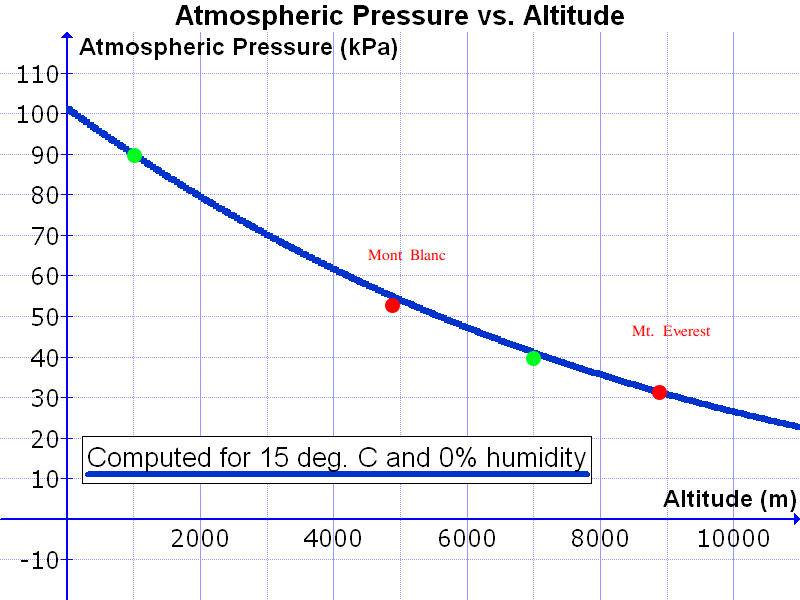
\includegraphics[width=0.7\linewidth]{figures/Atmospheric_Pressure_vs._Altitude.png}
\caption{Atmospheric pressure versus altitude (Wikipedia). Green points
represent our measurements, red points represent
interpolation/extrapolation.}
\label{fig:Pvsh}
\end{figure}

\subsection{Limitations of Interpolation}
Interpolation is just an approximation and works well when either the function $f$ is linear or we are trying to interpolate between two points that are close enough to believe that $f$ is almost linear in that interval.

It can be easily demonstrated that the linear approximation between two points of a given function $f(x)$ gets worse with the second derivative of the function that is approximated ($f''(x)$). This is intuitively correct: the "curvier" the function is, the worse the approximation made with simple linear interpolation becomes, see Fig.~\ref{fig:sine_interp} where we try to interpolate a sine function.

\begin{figure}
  \centering
  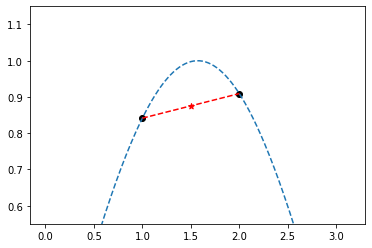
\includegraphics[width=0.7\textwidth]{figures/wrong_interp.png}
  \caption{Trying to approximate a sine function with a line is clearly not going to work unless the interpolation interval is very small.}
  \label{fig:sine_interp}
\end{figure}

To improve the approximation accuracy with complicated curves a polynomial of higher order can be used ($𝑝(𝑥)=𝑎_0 + 𝑎_1 𝑥+ 𝑎_2 𝑥^2+\cdots$), for example in the evaluation of the natural logarithm and trigonometric functions. It has to be clear however that going to higher degrees does not always help~\cite{bib:runge}.

\section{Discount Curve Interpolation}\label{discount-curve-interpolation}

Finally we can come back to finance. Since discount factors are derived from a 
discrete set of dates we may need to find the factor at some different date and 
clearly we can use interpolation to do it.
Now we will see how to implement a \texttt{python} function which interpolates some 
given discount factors.
To complete such a task we need:

\begin{itemize}
\tightlist
\item a list of pillars dates specifying the value dates of the given discount factors, \(t_0,...,t_{n-1}\);
\item a list of given discount factors, \(D(t_0),...,D(t_{n-1})\);
\item a pricing date (`today' date) which corresponds to \(t=0\).
\end{itemize}

The input argument to the function will be the value date at which we want to interpolate the discount factor. Since the discount factor can be expressed as \(D=e^{-r(T-t)}\) the function will use a log-linear interpolation to return the value at a date not included in the given pillars:

\begin{equation}
\begin{gathered}
d(t_i)=\mathrm{ln}(D(t_i))\\
d(t) = (1-w)d(t_i) + wd(t_{i+1});\quad w=\frac{t-t_i}{t_{i+1}-t_i}\\
D(t) = \mathrm{exp}(d(t))
\end{gathered}
\end{equation}
where \(i\) is such that \(t_i \le t \le t_{i+1}\)

Instead of reinventing the wheel and performing the interpolation with our own code, 
we'll use the function \texttt{interp} provided by the module \texttt{numpy}. 
This function linearly interpolates between the provided points to estimate the value 
of $f$ at some "new" $x$.
Say we want to interpolate the points at $x = 2.5$ given the following values:

\begin{codebox}
\begin{Verbatim}[commandchars=\\\{\}]
\PY{k+kn}{import} \PY{n+nn}{numpy} \PY{k}{as} \PY{n+nn}{np}

\PY{n}{xp} \PY{o}{=} \PY{p}{[}\PY{l+m+mi}{0}\PY{p}{,} \PY{l+m+mi}{1}\PY{p}{,} \PY{l+m+mi}{5}\PY{p}{]}
\PY{n}{fp} \PY{o}{=} \PY{p}{[}\PY{l+m+mi}{0}\PY{p}{,} \PY{l+m+mi}{2}\PY{p}{,} \PY{l+m+mi}{4}\PY{p}{]}
\PY{n}{np}\PY{o}{.}\PY{n}{interp}\PY{p}{(}\PY{l+m+mf}{2.5}\PY{p}{,} \PY{n}{xp}\PY{p}{,} \PY{n}{fp}\PY{p}{)}

2.75
\end{Verbatim}
\end{codebox}

Since discount factors are an essential part for every financial calculation, using an object
oriented approach, we are going to define \texttt{python} class which manages discount factors
and curves.

This class, that we name \texttt{DiscountCurve}, should have as attributes the pillar dates 
with the corresponding discount factors and initially only a method to interpolate discount 
factors.

Of course in order to perform the interpolation we are going to use \texttt{numpy.interp} but
when dealing with discount factors we need to be careful. Indeed \texttt{numpy.interp} only 
accepts numbers or a list of numbers as argument i.e. it doesn't automatically convert or 
interpret dates as numbers and doesn't know how to interpolate them. So we need to do 
the conversion ourselves before passing any dates to the interpolation function.
That's why in the constructor there is \texttt{pillar\_days} i.e. each date is replaced 
by the number of days from today ($t_0$).

Furthermore we also attempted a simple optimization of the code, in the class constructor indeed
we are going to apply the logarithm already to the input discount factors, so that we can save
some computation time with respect to doing the log at every call of \texttt{df}. 

\begin{codebox}
\begin{Verbatim}[commandchars=\\\{\}]
\PY{k+kn}{import} \PY{n+nn}{math}
\PY{k+kn}{import} \PY{n+nn}{numpy}
\PY{k+kn}{from} \PY{n+nn}{datetime} \PY{k}{import} \PY{n}{date}
	
\PY{k}{class} \PY{n+nc}{DiscountCurve}\PY{p}{:}	
    \PY{k}{def} \PY{n+nf}{\PYZus{}\PYZus{}init\PYZus{}\PYZus{}}\PY{p}{(}\PY{n+nb+bp}{self}\PY{p}{,} \PY{n}{today}\PY{p}{,} \PY{n}{pillar\PYZus{}dates}\PY{p}{,} \PY{n}{discount\PYZus{}factors}\PY{p}{)}\PY{p}{:}
        \PY{n+nb+bp}{self}\PY{o}{.}\PY{n}{today} \PY{o}{=} \PY{n}{today}
        \PY{n+nb+bp}{self}\PY{o}{.}\PY{n}{pillar\PYZus{}dates} \PY{o}{=} \PY{n}{pillar\PYZus{}dates}
        \PY{n+nb+bp}{self}\PY{o}{.}\PY{n}{discount\PYZus{}factors} \PY{o}{=} \PY{n}{discount\PYZus{}factors}
        \PY{n+nb+bp}{self}\PY{o}{.}\PY{n}{log\PYZus{}discount\PYZus{}factors} \PY{o}{=} \PY{p}{[}\PY{n}{math}\PY{o}{.}\PY{n}{log}\PY{p}{(}\PY{n}{discount\PYZus{}factor}\PY{p}{)} \PYZbs{}
            \PY{k}{for} \PY{n}{discount\PYZus{}factor} \PY{o+ow}{in} \PY{n+nb+bp}{self}\PY{o}{.}\PY{n}{discount\PYZus{}factors}\PY{p}{]}
        \PY{n+nb+bp}{self}\PY{o}{.}\PY{n}{pillar\PYZus{}days} \PY{o}{=} \PY{p}{[}\PY{p}{(}\PY{n}{pillar\PYZus{}date} \PY{o}{\PYZhy{}} \PY{n+nb+bp}{self}\PY{o}{.}\PY{n}{today}\PY{p}{)}\PY{o}{.}\PY{n}{days} \PYZbs{}
            \PY{k}{for} \PY{n}{pillar\PYZus{}date} \PY{o+ow}{in} \PY{n+nb+bp}{self}\PY{o}{.}\PY{n}{pillar\PYZus{}dates}\PY{p}{]}

    \PY{k}{def} \PY{n+nf}{df}\PY{p}{(}\PY{n+nb+bp}{self}\PY{p}{,} \PY{n}{d}\PY{p}{)}\PY{p}{:}
        \PY{n}{d\PYZus{}days} \PY{o}{=} \PY{p}{(}\PY{n}{d} \PY{o}{\PYZhy{}} \PY{n+nb+bp}{self}\PY{o}{.}\PY{n}{today}\PY{p}{)}\PY{o}{.}\PY{n}{days}
        \PY{n}{interp\PYZus{}log\PYZus{}df} \PY{o}{=} \PYZbs{}
            \PY{n}{numpy}\PY{o}{.}\PY{n}{interp}\PY{p}{(}\PY{n}{d\PYZus{}days}\PY{p}{,} \PY{n+nb+bp}{self}\PY{o}{.}\PY{n}{pillar\PYZus{}days}\PY{p}{,} \PY{n+nb+bp}{self}\PY{o}{.}\PY{n}{log\PYZus{}discount\PYZus{}factors}\PY{p}{)}
        \PY{k}{return} \PY{n}{math}\PY{o}{.}\PY{n}{exp}\PY{p}{(}\PY{n}{interp\PYZus{}log\PYZus{}df}\PY{p}{)}
\end{Verbatim}
\end{codebox}

This class is going to be the first step in the creation of a \texttt{python} financial library,
so copy the code into a separate file called \texttt{finmarkets.py} so that you can later reuse 
its code.

Assume we have three discount factors, we can now use our new class to create the corresponding
discount curve. Then we can use the \texttt{df} method of this class to get discount factors 
on value dates between the given pillar dates.

\begin{codebox}
\begin{Verbatim}[commandchars=\\\{\}]
\PY{k+kn}{from} \PY{n+nn}{datetime} \PY{k}{import} \PY{n}{date}
\PY{k+kn}{from} \PY{n+nn}{finmarkets} \PY{k}{import} \PY{n}{DiscountCurve}
	
\PY{n}{today\PYZus{}date} \PY{o}{=} \PY{n}{date}\PY{p}{(}\PY{l+m+mi}{2019}\PY{p}{,} \PY{l+m+mi}{10}\PY{p}{,} \PY{l+m+mi}{1}\PY{p}{)}
	
\PY{n}{pillar\PYZus{}dates} \PY{o}{=} \PY{p}{[}\PY{n}{date}\PY{p}{(}\PY{l+m+mi}{2019}\PY{p}{,} \PY{l+m+mi}{10}\PY{p}{,} \PY{l+m+mi}{1}\PY{p}{)}\PY{p}{,} \PY{n}{date}\PY{p}{(}\PY{l+m+mi}{2020}\PY{p}{,} \PY{l+m+mi}{10}\PY{p}{,} \PY{l+m+mi}{1}\PY{p}{)}\PY{p}{,} \PY{n}{date}\PY{p}{(}\PY{l+m+mi}{2021}\PY{p}{,} \PY{l+m+mi}{10}\PY{p}{,} \PY{l+m+mi}{1}\PY{p}{)}\PY{p}{]}
\PY{n}{discount\PYZus{}factors} \PY{o}{=} \PY{p}{[}\PY{l+m+mf}{1.0}\PY{p}{,} \PY{l+m+mf}{0.97}\PY{p}{,} \PY{l+m+mf}{0.72}\PY{p}{]}

\PY{n}{curve} \PY{o}{=} \PY{n}{DiscountCurve}\PY{p}{(}\PY{n}{today\PYZus{}date}\PY{p}{,} \PY{n}{pillar\PYZus{}dates}\PY{p}{,} \PY{n}{discount\PYZus{}factors}\PY{p}{)}
\PY{n}{d0} \PY{o}{=} \PY{n}{date}\PY{p}{(}\PY{l+m+mi}{2020}\PY{p}{,} \PY{l+m+mi}{1}\PY{p}{,} \PY{l+m+mi}{1}\PY{p}{)}
\PY{n}{df0} \PY{o}{=} \PY{n}{curve.df}\PY{p}{(}\PY{n}{d0, today_date, pillar_dates, discount_factors}\PY{p}{)}
\PY{n+nb}{print} \PY{p}{(}\PY{n}{df0}\PY{p}{)}

0.9923728228571693

\PY{n}{d1} \PY{o}{=} \PY{n}{date}\PY{p}{(}\PY{l+m+mi}{2021}\PY{p}{,} \PY{l+m+mi}{1}\PY{p}{,} \PY{l+m+mi}{1}\PY{p}{)}
\PY{n}{df1} \PY{o}{=} \PY{n}{curve.df}\PY{p}{(}\PY{n}{d1, today_date, pillar_dates, discount_factors}\PY{p}{)}
\PY{n+nb}{print} \PY{p}{(}\PY{n}{df1}\PY{p}{)}

0.8997999273630835
\end{Verbatim}
\end{codebox}

A very useful way to check the correctness of a result is by plotting it. So let's see what this looks like when plotted on a semi-log graph and if it makes sense, Fig.~\ref{fig:log_discount_curve}.

\begin{codebox}
\begin{Verbatim}[commandchars=\\\{\}]
\PY{k+kn}{from} \PY{n+nn}{matplotlib} \PY{k}{import} \PY{n}{pyplot} \PY{k}{as} \PY{n}{plt}
\PY{k+kn}{import} \PY{n+nn}{matplotlib}\PY{n+nn}{.}\PY{n+nn}{dates} \PY{k}{as} \PY{n+nn}{mdates}
	
\PY{n}{plt}\PY{o}{.}\PY{n}{plot}\PY{p}{(}\PY{n}{pillar\PYZus{}dates}\PY{p}{,} \PY{n}{discount\PYZus{}factors}\PY{p}{,} \PY{n}{marker}\PY{o}{=}\PY{l+s+s1}{\PYZsq{}}\PY{l+s+s1}{o}\PY{l+s+s1}{\PYZsq{}}\PY{p}{)}
\PY{n}{plt}\PY{o}{.}\PY{n}{plot}\PY{p}{(}\PY{n}{d0}\PY{p}{,} \PY{n}{df0}\PY{p}{,} \PY{n}{marker}\PY{o}{=}\PY{l+s+s1}{\PYZsq{}}\PY{l+s+s1}{X}\PY{l+s+s1}{\PYZsq{}}\PY{p}{)}
\PY{n}{plt}\PY{o}{.}\PY{n}{plot}\PY{p}{(}\PY{n}{d1}\PY{p}{,} \PY{n}{df1}\PY{p}{,} \PY{n}{marker}\PY{o}{=}\PY{l+s+s1}{\PYZsq{}}\PY{l+s+s1}{X}\PY{l+s+s1}{\PYZsq{}}\PY{p}{)}
\PY{n}{plt}\PY{o}{.}\PY{n}{gca}\PY{p}{(}\PY{p}{)}\PY{o}{.}\PY{n}{xaxis}\PY{o}{.}\PY{n}{set\PYZus{}major\PYZus{}formatter}\PY{p}{(}\PY{n}{mdates}\PY{o}{.}\PY{n}{DateFormatter}\PY{p}{(}\PY{l+s+s1}{\PYZsq{}}\PY{l+s+s1}{\PYZpc{}}\PY{l+s+s1}{m/}\PY{l+s+si}{\PYZpc{}d}\PY{l+s+s1}{/}\PY{l+s+s1}{\PYZpc{}}\PY{l+s+s1}{Y}\PY{l+s+s1}{\PYZsq{}}\PY{p}{)}\PY{p}{)}
\PY{n}{plt}\PY{o}{.}\PY{n}{gca}\PY{p}{(}\PY{p}{)}\PY{o}{.}\PY{n}{xaxis}\PY{o}{.}\PY{n}{set\PYZus{}major\PYZus{}locator}\PY{p}{(}\PY{n}{mdates}\PY{o}{.}\PY{n}{YearLocator}\PY{p}{(}\PY{p}{)}\PY{p}{)}
\PY{n}{plt}\PY{o}{.}\PY{n}{grid}\PY{p}{(}\PY{k+kc}{True}\PY{p}{)}
\PY{n}{plt}\PY{o}{.}\PY{n}{yscale}\PY{p}{("log"}\PY{p}{)}
\PY{n}{plt}\PY{o}{.}\PY{n}{show}\PY{p}{(}\PY{p}{)}
\end{Verbatim}
\end{codebox}

\begin{figure}[htb]
	\centering
	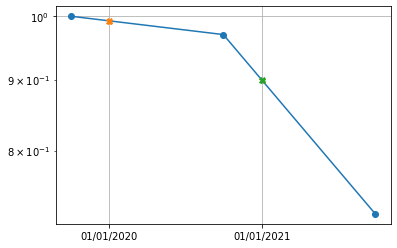
\includegraphics[width=0.7\textwidth]{figures/log_discount_curve}
	\caption{Plot of the discount curve defined in the text and of the two computed
		discount factors with semi-log scale.}
	\label{fig:log_discount_curve}
\end{figure}

Let's see what it looks like when plotted on a linear graph too, Fig.~\ref{fig:linear_discount_curve}.

\begin{codebox}
\begin{Verbatim}[commandchars=\\\{\}]
\PY{n}{plt}\PY{o}{.}\PY{n}{plot}\PY{p}{(}\PY{n}{pillar\PYZus{}dates}\PY{p}{,} \PY{n}{discount\PYZus{}factors}\PY{p}{,} \PY{n}{marker}\PY{o}{=}\PY{l+s+s1}{\PYZsq{}}\PY{l+s+s1}{o}\PY{l+s+s1}{\PYZsq{}}\PY{p}{)}
\PY{n}{plt}\PY{o}{.}\PY{n}{plot}\PY{p}{(}\PY{n}{d0}\PY{p}{,} \PY{n}{df0}\PY{p}{,} \PY{n}{marker}\PY{o}{=}\PY{l+s+s1}{\PYZsq{}}\PY{l+s+s1}{X}\PY{l+s+s1}{\PYZsq{}}\PY{p}{)}
\PY{n}{plt}\PY{o}{.}\PY{n}{plot}\PY{p}{(}\PY{n}{d1}\PY{p}{,} \PY{n}{df1}\PY{p}{,} \PY{n}{marker}\PY{o}{=}\PY{l+s+s1}{\PYZsq{}}\PY{l+s+s1}{X}\PY{l+s+s1}{\PYZsq{}}\PY{p}{)}
\PY{n}{plt}\PY{o}{.}\PY{n}{gca}\PY{p}{(}\PY{p}{)}\PY{o}{.}\PY{n}{xaxis}\PY{o}{.}\PY{n}{set\PYZus{}major\PYZus{}formatter}\PY{p}{(}\PY{n}{mdates}\PY{o}{.}\PY{n}{DateFormatter}\PY{p}{(}\PY{l+s+s1}{\PYZsq{}}\PY{l+s+s1}{\PYZpc{}}\PY{l+s+s1}{m/}\PY{l+s+si}{\PYZpc{}d}\PY{l+s+s1}{/}\PY{l+s+s1}{\PYZpc{}}\PY{l+s+s1}{Y}\PY{l+s+s1}{\PYZsq{}}\PY{p}{)}\PY{p}{)}
\PY{n}{plt}\PY{o}{.}\PY{n}{gca}\PY{p}{(}\PY{p}{)}\PY{o}{.}\PY{n}{xaxis}\PY{o}{.}\PY{n}{set\PYZus{}major\PYZus{}locator}\PY{p}{(}\PY{n}{mdates}\PY{o}{.}\PY{n}{YearLocator}\PY{p}{(}\PY{p}{)}\PY{p}{)}
\PY{n}{plt}\PY{o}{.}\PY{n}{grid}\PY{p}{(}\PY{k+kc}{True}\PY{p}{)}
\PY{n}{plt}\PY{o}{.}\PY{n}{show}\PY{p}{(}\PY{p}{)}
\end{Verbatim}
\end{codebox}

\begin{figure}[htb]
	\centering
	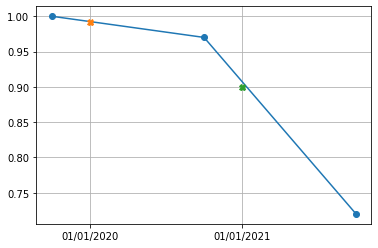
\includegraphics[width=0.7\textwidth]{figures/linear_discount_curve}
	\caption{Plot of the discount curve defined in the text and of the two computed
		discount factors with linear scale.}
	\label{fig:linear_discount_curve}
\end{figure}
\noindent
Discrepancies in the linear plot are most likely due to rounding.

\section{Forward Rates}\label{calculating-forward-rates}
A forward rate is an interest rate applicable to a financial transaction that will 
take place in the future. It can be considered to be the market's expectations for 
future prices and can serve as an indicator of how the market expects the future to perform.

Instead the \emph{spot rate} is used by buyers and sellers looking 
to make an immediate purchase or sale, and it cannot be an indicator of market 
expectations.

Forward rates are calculated from the spot rate by exploiting the no arbitrage condition which states that investing at rate \(r_1\) for the period \((0, T_1)\) and then \emph{re-investing} at rate \(r_{1,2}\) for the time period \((T_1, T_2)\) is equivalent to invest at rate \(r_2\) for the full time period \((0, T_2)\). Essentially two investors shouldn't be able to earn money from arbitraging between different interest periods. That said:

\begin{equation}
(1+r_1 T_1)(1+r_{1,2}(T_2 - T_1)) = 1 + r_2 T_2
\label{eq:no_arbitrage_r}
\end{equation}
Solving for \(r_{1,2}\) leads to

\begin{equation}
F(T_1, T_2) = r_{1,2} = \frac{1}{T_2 - T_1}\Big(\frac{1+r_2 T_2}{1+r_1 T_1} - 1 \Big)
\label{eq:forward_rate_simple}
\end{equation}
\vspace{0.5cm}
The same expression in terms of the discount factor $ D{(0, T_i)}=\cfrac{1}{1+r_iT_{i}}$ becomes
\begin{equation}
F(T_1, T_2) = \frac{1}{T_2 - T_1}\Big(\frac{D(0, T_1)}{D(0, T_2)} - 1 \Big)
\end{equation}
Considering continuously compounded rates Eq.~\ref{eq:no_arbitrage_r} can be
written as
\begin{equation*}
e^{{(r}_{2}T_{2})}=e^{{(r}_{1}T_{1})}\ast \ e^{\left(r_{1,2} \left(T_{2}-T_{1}\right)\right)}
\end{equation*}
and the corresponding expression for the forward rate is
\begin{equation}
F(T_1, T_2) = r_{1,2} = \frac {1}{T_{2}-T_{1}}(\ln D(0,T_{1})-\ln D(0,T_{2}))
\quad(\textrm{since now } D(0, T_i)=e^{-r_i T_i})
\label{eq:forward_rate_continous}
\end{equation}

We now write a very simple \texttt{ForwardRateCurve} class which doesn't compute 
discount factors or other fancy values but it is just a container for a list 
of forward rates and can interpolates between them.
Also this class goes into the \texttt{finmarkets} module and will be used to
define the LIBOR curve needed throughout future Chapters.

In this case it is enough to write a new class that has three attributes: 
a set of pillar dates and the corresponding forward rates. The reference date to convert 
the pillars for the interpolation (i.e. today) is taken from the first item of the pillar list.
There will be just a single method \texttt{forward\_rate} to return an interpolated rate.

\begin{codebox}[size=fbox, boxrule=1pt, colback=cellbackground, colframe=cellborder]
\begin{Verbatim}[commandchars=\\\{\}]
\PY{k+kn}{import} \PY{n+nn}{numpy}
	
\PY{k}{class} \PY{n+nc}{ForwardRateCurve}\PY{p}{(}\PY{n+nb}{object}\PY{p}{)}\PY{p}{:}	
    \PY{k}{def} \PY{n+nf}{\PYZus{}\PYZus{}init\PYZus{}\PYZus{}}\PY{p}{(}\PY{n+nb+bp}{self}\PY{p}{,} \PY{n}{pillar\PYZus{}dates}\PY{p}{,} \PY{n}{rates}\PY{p}{)}\PY{p}{:}
        \PY{n+nb+bp}{self}\PY{o}{.}\PY{n}{today} \PY{o}{=} \PY{n}{pillar\PYZus{}dates}\PY{p}{[}\PY{l+m+mi}{0}\PY{p}{]}
        \PY{n+nb+bp}{self}\PY{o}{.}\PY{n}{rates} \PY{o}{=} \PY{n}{rates}
        \PY{n+nb+bp}{self}\PY{o}{.}\PY{n}{pillar\PYZus{}days} \PY{o}{=} \PY{p}{[}\PY{p}{(}\PY{n}{pillar\PYZus{}date} \PY{o}{\PYZhy{}} \PY{n+nb+bp}{self}\PY{o}{.}\PY{n}{today}\PY{p}{)}\PY{o}{.}\PY{n}{days} \PYZbs{}
            \PY{k}{for} \PY{n}{pillar\PYZus{}date} \PY{o+ow}{in} \PY{n}{pillar\PYZus{}dates}\PY{p}{]}
	
    \PY{k}{def} \PY{n+nf}{forward\PYZus{}rate}\PY{p}{(}\PY{n+nb+bp}{self}\PY{p}{,} \PY{n}{d}\PY{p}{)}\PY{p}{:}
        \PY{n}{d\PYZus{}days} \PY{o}{=} \PY{p}{(}\PY{n}{d} \PY{o}{\PYZhy{}} \PY{n+nb+bp}{self}\PY{o}{.}\PY{n}{today}\PY{p}{)}\PY{o}{.}\PY{n}{days}
        \PY{k}{return} \PY{n}{numpy}\PY{o}{.}\PY{n}{interp}\PY{p}{(}\PY{n}{d\PYZus{}days}\PY{p}{,} \PY{n+nb+bp}{self}\PY{o}{.}\PY{n}{pillar\PYZus{}days}\PY{p}{,} \PY{n+nb+bp}{self}\PY{o}{.}\PY{n}{rates}\PY{p}{)}
\end{Verbatim}
\end{codebox}

\section{Multi-curve Framework}
\label{sec:financial-crisis}

Prior to the 2008 financial crisis, interbank deposits posed little 
credit/liquidity issues, interbank lending rates (IBOR rates, e.g. LIBOR, EURIBOR)
were essentially a good proxy for risk free rates. 
Basis swap spreads were negligible and thereby neglected. 

Looking at the historical series of the EURIBOR (6M) rate versus the EONIA 
Overnight Indexed Swap (OIS-6M) rate over the time interval 2006-2011 in Fig.~\ref{fig:credit_crunch} it becomes
apparent how before August 2007 the two rates display strictly overlapping trends differing of no more than 6 bps.

\begin{figure}[htb]
	\centering
	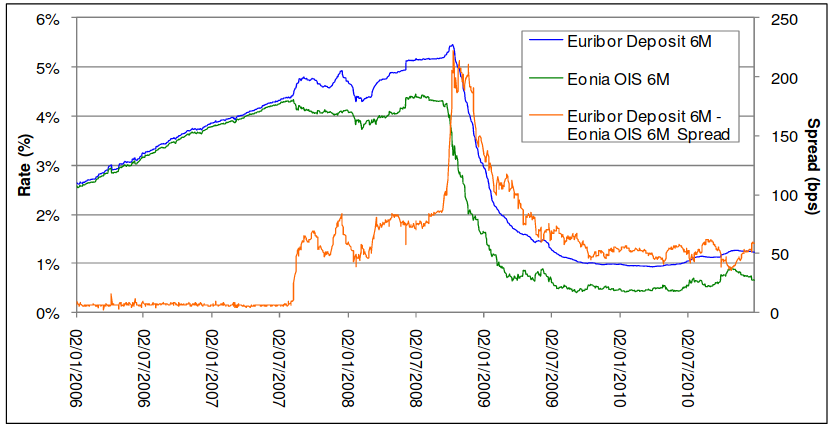
\includegraphics[width=0.9\linewidth]{figures/credit_crunch.png}
	\caption{Historical series of EURIBOR 6M rate versus EONIA OIS 6M rate. The corresponding spread 
		is shown on the right axis (Jan. 06 - Dec. 10 window, source: Bloomberg).}
	\label{fig:credit_crunch}
\end{figure}

A single yield curve constructed out of selected deposit rates, FRA/EDF rates 
and swap rates served both the cash flow projection and discounting purposes.

During the 2008 financial crisis, the failure of some banks however proved that interbank lending rates (e.g. LIBOR, EURIBOR\ldots) were not risk-free. Meanwhile
there was also significant counterparty credit risk arising from derivative
transactions that were not subject to collateral or margin calls. 
Basis swap spreads greatly widened, and persist to this day. 

Still looking at Fig.~\ref{fig:credit_crunch} it is clear how in August 2007
a sudden increase of the EURIBOR rate and a simultaneous decrease of the OIS rate
leads to the explosion of the corresponding basis spread, touching the peak of 222
bps in October 2008, when Lehman Brothers filed for bankruptcy. Successively the
basis has sensibly reduced and stabilized between 40 bps and 60 bps (notice that the precrisis 
level has never been recovered). 
The same effect is observed for other similar couples of series, e.g. EURIBOR 3M 
vs OIS 3M.

The existence of such significant basis swap spreads reflects the fact that after
the crisis the interest rate market has been segmented into subareas corresponding
to instruments with different underlying rate tenors, characterized by different 
rate dynamics. 

Traditional single curve based pricing approach ignores these differences. 
It mixes different underlying rate tenors and incorporates different rate dynamics,
eventually leads to inconsistency.
After the crisis, the market practice has thus evolved to take into account the new
market information (e.g. the basis swap spreads, collateralization, etc.), that
translate into the additional requirement of homogeneity and funding. 
The homogeneity requirement means that interest rate derivatives with a given
underlying rate tenor must be priced and hedged using vanilla interest rate
market instruments with the same underlying. The funding requirement means that 
the discount rate of any cash flow generated by the derivative must be consistent, 
by no-arbitrage, with the funding rate associated with that cash flow. 

Driven by the crisis, many derivative contracts have been updated to include permissible credit mitigants for a transaction, such as netting and collateralization in cash.
Since standard agreements stipulate daily margination on collateral and the cash
collateral earns a return at overnight rate,
overnight rate becomes a natural choice for the risk-free discount rate or
the funding rate. This is referred to as \emph{OIS discounting}.

The large spread between risk free rate and interbank lending rate during and after
2008 financial crisis it is not possible anymore to use a single curve for
discounting and derivative valuation. The traditional single curve used for both 
cash flow projection and discounting turned out to be obsolete. The markets
have since nearly switched to multi-curve framework. 

For example, if we want to calculate the net present value (NPV) of a forward 6-month 
LIBOR coupon, we need to simultaneously use two different discount curves:

\begin{itemize}
\tightlist
\item the 6-month LIBOR curve for determining the forward rate;
\item the EONIA curve for discounting the expected cash flow.
\end{itemize}

%The reason of the abrupt divergence between the Euribor and OIS rates can be explained by considering both the monetary policy decisions adopted by international authorities in response to the financial turmoil, and the impact of the credit crunch on both credit and liquidity risk perception of the market, coupled with the different financial meaning and dynamics of these rates.

%\begin{itemize}
%\tightlist
%\item
%  The Euribor rate is the reference rate for over-the-counter (OTC)
%  transactions in the Euro area. It is defined as the rate at which
%  Euro inter-bank deposits are being offered within the EMU zone by one
%  prime bank to another at 11:00 a.m. Brussels time. The rate fixings
%  for a strip of 15 maturities (from one day to one year) are
%  constructed as the average of the rates submitted (excluding the
%  highest and lowest 15\% tails) by a panel of 42 banks, selected
%  among the EU banks with the highest volume of business in the Euro
%  zone money markets, plus some large international bank from non-EU
%  countries with important euro zone operations. \emph{Thus, Euribor
%  rates reflect the average cost of funding of banks in the inter bank
%  market at each given maturity. During the crisis the solvency and
%  solidity of the whole financial sector was brought into question and
%  the credit and liquidity risk and uremia associated to inter-bank
%  counter-parties sharply increased.} The Euribor rates immediately
%  reflected these dynamics and raise to their highest values over more
%  than 10 years. As seen in the plot above, the Euribor 6M rate suddenly
%  increased on August 2007 and reached 5.49\% on 10th October 2008.
%\item
%  The EONIA rate is the reference rate for overnight OTC transactions in
%  the Euro area. It is constructed as the average rate of the overnight
%  transactions (one day maturity deposits) executed during a given
%  business day by a panel of banks on the inter-bank money market,
%  weighted with the corresponding transaction volumes. \emph{The EONIA
%  Contribution Panel coincides with the Euribor Contribution Panel, thus
%  EONIA rate includes information on the short term (overnight)
%  liquidity expectations of banks in the Euro money market. It is also
%  used by the European Central Bank (ECB) as a method of effecting and
%  observing the transmission of its monetary policy actions. During the
%  crisis the central banks were mainly concerned about stabilizing the
%  level of liquidity in the market, thus they reduced the level of the
%  official rates.} Furthermore, the daily tenor of the EONIA rate makes
%  negligible the credit and liquidity risks reflected on it: for this
%  reason the OIS rates are considered the best proxies available in the
%  market for the risk-free rate.
%\end{itemize}

Our financial library has to implement the following calculation

\[\mathrm{NPV} = D_{\mathrm{EONIA}}(T_1) \cdot \frac{1}{T_2-T_1}\Big(\frac{D_{\mathrm{LIBOR}}(T_1)}{D_{\mathrm{LIBOR}}(T_2)} - 1 \Big)\]
\noindent
In order to do so we can extend the \texttt{DiscountCurve} class with a \texttt{forward\_rate}
method

\begin{codebox}
\begin{Verbatim}[commandchars=\\\{\}]
\PY{k}{class} \PY{n+nc}{DiscountCurve}\PY{p}{:}	
    ...
    \PY{k}{def} \PY{n+nf}{forward\PYZus{}rate}\PY{p}{(}\PY{n+nb+bp}{self}\PY{p}{,} \PY{n}{d1}\PY{p}{,} \PY{n}{d2}\PY{p}{)}\PY{p}{:}
        \PY{k}{return} \PY{p}{(}\PY{n+nb+bp}{self}\PY{o}{.}\PY{n}{df}\PY{p}{(}\PY{n}{d1}\PY{p}{)} \PY{o}{/} \PY{n+nb+bp}{self}\PY{o}{.}\PY{n}{df}\PY{p}{(}\PY{n}{d2}\PY{p}{)} \PY{o}{\PYZhy{}} \PY{l+m+mf}{1.0}\PY{p}{)} \PY{o}{*} \PYZbs{}
	        \PY{p}{(}\PY{l+m+mf}{365.0} \PY{o}{/} \PY{p}{(}\PY{p}{(}\PY{n}{d2} \PY{o}{\PYZhy{}} \PY{n}{d1}\PY{p}{)}\PY{o}{.}\PY{n}{days}\PY{p}{)}\PY{p}{)}
\end{Verbatim}
\end{codebox}

As an example let's define EONIA and LIBOR curves and compute the net present value 
of the forward 6-month LIBOR coupon mentioned before.

\begin{codebox}
\begin{Verbatim}[commandchars=\\\{\}]
\PY{k+kn}{from} \PY{n+nn}{finmarkets} \PY{k}{import} \PY{n}{DiscountCurve}
	
\PY{n}{today\PYZus{}date} \PY{o}{=} \PY{n}{date} \PY{p}{(}\PY{l+m+mi}{2020}\PY{p}{,} \PY{l+m+mi}{1}\PY{p}{,} \PY{l+m+mi}{1}\PY{p}{)}
\PY{n}{t1} \PY{o}{=} \PY{n}{date}\PY{p}{(}\PY{l+m+mi}{2020}\PY{p}{,} \PY{l+m+mi}{4}\PY{p}{,} \PY{l+m+mi}{1}\PY{p}{)}
\PY{n}{t2} \PY{o}{=} \PY{n}{date}\PY{p}{(}\PY{l+m+mi}{2020}\PY{p}{,} \PY{l+m+mi}{10}\PY{p}{,} \PY{l+m+mi}{1}\PY{p}{)}

\PY{n}{pillar\PYZus{}dates\PYZus{}eonia} \PY{o}{=} \PY{p}{[}\PY{n}{date}\PY{p}{(}\PY{l+m+mi}{2020}\PY{p}{,} \PY{l+m+mi}{1}\PY{p}{,} \PY{l+m+mi}{1}\PY{p}{)}\PY{p}{,} \PY{n}{date}\PY{p}{(}\PY{l+m+mi}{2021}\PY{p}{,} \PY{l+m+mi}{1}\PY{p}{,} \PY{l+m+mi}{1}\PY{p}{)}\PY{p}{,} \PY{n}{date}\PY{p}{(}\PY{l+m+mi}{2022}\PY{p}{,} \PY{l+m+mi}{10} \PY{p}{,}\PY{l+m+mi}{1}\PY{p}{)}\PY{p}{]}
\PY{n}{df\PYZus{}eonia} \PY{o}{=} \PY{p}{[}\PY{l+m+mf}{1.0}\PY{p}{,} \PY{l+m+mf}{0.97}\PY{p}{,} \PY{l+m+mf}{0.72}\PY{p}{]}
	
\PY{n}{pillar\PYZus{}dates\PYZus{}libor} \PY{o}{=} \PY{p}{[}\PY{n}{date}\PY{p}{(}\PY{l+m+mi}{2020}\PY{p}{,} \PY{l+m+mi}{1}\PY{p}{,} \PY{l+m+mi}{1}\PY{p}{)}\PY{p}{,} \PY{n}{date}\PY{p}{(}\PY{l+m+mi}{2020}\PY{p}{,} \PY{l+m+mi}{6}\PY{p}{,} \PY{l+m+mi}{1}\PY{p}{)}\PY{p}{,} \PY{n}{date}\PY{p}{(}\PY{l+m+mi}{2020}\PY{p}{,} \PY{l+m+mi}{12} \PY{p}{,}\PY{l+m+mi}{1}\PY{p}{)}\PY{p}{]}
\PY{n}{df\PYZus{}libor} \PY{o}{=} \PY{p}{[}\PY{l+m+mf}{1.0}\PY{p}{,} \PY{l+m+mf}{0.95}\PY{p}{,} \PY{l+m+mf}{0.90}\PY{p}{]}
		
\PY{n}{eonia\PYZus{}curve} \PY{o}{=} \PY{n}{DiscountCurve}\PY{p}{(}\PY{n}{today\PYZus{}date}\PY{p}{,} \PY{n}{pillar\PYZus{}dates\PYZus{}eonia}\PY{p}{,} \PY{n}{df\PYZus{}eonia}\PY{p}{)}
\PY{n}{libor\PYZus{}curve} \PY{o}{=} \PY{n}{DiscountCurve}\PY{p}{(}\PY{n}{today\PYZus{}date}\PY{p}{,} \PY{n}{pillar\PYZus{}dates\PYZus{}libor}\PY{p}{,} \PY{n}{df\PYZus{}libor}\PY{p}{)}
	
\PY{n}{npv} \PY{o}{=} \PY{n}{eonia\PYZus{}curve}\PY{o}{.}\PY{n}{df}\PY{p}{(}\PY{n}{t1}\PY{p}{)} \PY{o}{*} \PY{n}{libor\PYZus{}curve}\PY{o}{.}\PY{n}{forward\PYZus{}rate}\PY{p}{(}\PY{n}{t1}\PY{p}{,} \PY{n}{t2}\PY{p}{)}
\PY{n}{npv\PYZus{}pre2008} \PY{o}{=} \PY{n}{libor\PYZus{}curve}\PY{o}{.}\PY{n}{df}\PY{p}{(}\PY{n}{t1}\PY{p}{)} \PY{o}{*} \PY{n}{libor\PYZus{}curve}\PY{o}{.}\PY{n}{forward\PYZus{}rate}\PY{p}{(}\PY{n}{t1}\PY{p}{,} \PY{n}{t2}\PY{p}{)}
	
\PY{n+nb}{print} \PY{p}{(}\PY{l+s+s2}{\PYZdq{}}\PY{l+s+s2}{NPV post 2008:}\PY{l+s+s2}{\PYZdq{}}\PY{p}{,} \PY{n}{npv}\PY{p}{)}
\PY{n+nb}{print} \PY{p}{(}\PY{l+s+s2}{\PYZdq{}}\PY{l+s+s2}{NPV pre 2008:}\PY{l+s+s2}{\PYZdq{}}\PY{p}{,} \PY{n}{npv\PYZus{}pre2008}\PY{p}{)}
	
NPV post 2008: 0.11533243116069992
NPV pre 2008: 0.11269481011359303
\end{Verbatim}
\end{codebox}

\subsection{Transitioning away from LIBOR~\cite{bib:str}}
A working group on euro risk-free rates was established to identify
and recommend risk-free rates that could serve as a basis for an
alternative to current benchmarks used in a variety of financial
instruments and contracts in the euro area, such as the euro
overnight index average (EONIA) and the euro interbank offered rate
(EURIBOR). 

The group recommended on September 2018 that the euro
short-term rate (STR) be used as the risk-free rate for the euro area
and is now focused on supporting the market with transitioning.
The ECB published the STR for the first time on 2nd October 2019,
reflecting trading activity on 1st October 2019.

The working group recommends that market participants should gradually replace
EONIA with the STR as a reference rate for all products and
contracts and make all necessary adjustments for using the STR as
their standard benchmark
The working group recommends the STR plus a fixed spread of 8.5
basis points as the EONIA fallback rate for all products and purposes.
The working group recommends that market participants should:
consider, whenever feasible and appropriate, no longer entering into
new contracts referencing EONIA, in particular new contracts
maturing after 31 December 2021, as EONIA will cease to exist after
that date.

The working group is also looking at identifying fallbacks for
EURIBOR based on the STR. Both backward and forward-looking
options are being considered. As part of its work on forward-looking
options, in March 2019 the working group recommended a
methodology based on (tradable) overnight index swap (OIS) quotes
for calculating a STR-based forward-looking term structure and later
invited benchmark administrators to express their interest in
producing such a term structure.

\begin{thebibliography}{9}
	%  %\bibitem{survey2019} StackOverflow \emph{The TEXbook}, Addison-Wesley, Reading,Massachusetts, second edition, 1984,
	\bibitem{bib:runge} \href{https://en.wikipedia.org/wiki/Runge\%27s_phenomenon}{\emph{Runge's phenomenon}}, Wikipedia [Online]
	\bibitem{bib:forward_rate}\href{https://www.investopedia.com/ask/answers/042315/what-difference-between-forward-rate-and-spot-rate.asp}{\emph{Forward Rate vs. Spot Rate: What's the Difference?}}, Investopedia [Online]
	\bibitem{bib:libor} \href{https://www.ig.com/it/glossario-trading/definizione-di-libor}{\emph{LIBOR}} [Online]
	\bibitem{bib:2008crisis} \href{https://www.investopedia.com/articles/economics/09/financial-crisis-review.asp}{\emph{The 2007-2008 Financial Crisis Review}}, Investopedia [Online]
	\bibitem{bib:str}
	B. Guggenheim and A. Schrimpf, 
	\href{https://www.bis.org/publ/work891.htm}{\emph{At the crossroads in the transition away from LIBOR - from overnight to term rates}}, BIS Working Papers No 891, 09 October 2020 [Online]
\end{thebibliography}
